\documentclass[12pt,a4paper]{report}
\usepackage[utf8]{inputenc}
\usepackage[english]{babel}
\usepackage{amsmath}
\usepackage{amsfonts}
\usepackage{amssymb}
\usepackage{graphicx}

\usepackage{tikz}
\usetikzlibrary{arrows,automata, positioning,calc}


\begin{document}


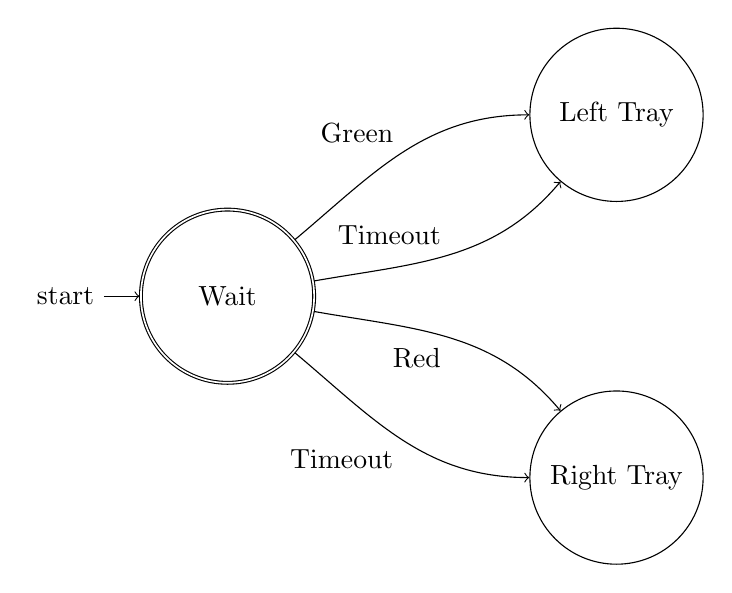
\begin{tikzpicture}[node distance=3cm]

\node[circle, minimum width=6cm, name=c] {};

\node[initial,accepting,state,name=start,minimum width=2.2cm] at (c.180)   {Wait}; 

\node[state,name=left,minimum width=2.2cm] at (c.50)   {Left Tray}; 
\node[state,name=right,minimum width=2.2cm] at (c.-50)   {Right Tray}; 


%\node[name=rst] at (-2.5,3) {rst};

\draw[->] (start) to[out=40, in=180] node[midway,above left] {Green} (left) ;
\draw[->] (start) to[out=10, in=230] node[midway,above left] {Timeout} (left) ;

\draw[->] (start) to[out=-10, in=-230] node[midway,below left] {Red} (right) ;
\draw[->] (start) to[out=-40, in=180] node[midway,below left] {Timeout} (right) ;

%\draw[->] (rst) to[out=-25, in=135] node[midway,above] {} (start) ;
 
 
\end{tikzpicture}


\end{document}